%% LaTeX2e class for student theses
%% thesis.tex
%% 
%% Original: https://www.overleaf.com/latex/templates/sdq-bachelor-slash-master-thesis-template-at-the-karlsruhe-institute-of-technology/fbncsmwspbgr with License (CC BY-NC) 4.0: free to share and adapt.

%% Karlsruhe Institute of Technology
%% Institute for Anthropomatics und Robotics (IAR)
%% Artificial Intelligence for Language Technologies (AI4LT) lab
%%
%% Prof. Dr. Jan Niehues
%% Lab's website https://ai4lt.anthropomatik.kit.edu/english/index.php

%% Available page modes: oneside, twoside (print setting)
%% Available languages: english, ngerman
% \documentclass[twoside, ngerman]{ai4ltthesis}
\documentclass[twoside, english]{ai4ltthesis}

%% ---------------------------------
%% | Information about the thesis  |
%% ---------------------------------

%% Name of the author
\author{Isabel Kraft}

%% Title (and possibly subtitle) of the thesis
\title{Unsupervised Quality Estimation in Spoken Language Translation with glass-box features}

%% Type of the thesis 
\thesistype{Bachelor's Thesis}

%% Change the institute here, ``AI4LT'' is default
% \myinstitute{Institute for \dots}



%% The reviewers are the professors that grade your thesis
\reviewerone{Prof. Dr. Jan Niehues}
\reviewertwo{Prof. Dr.-Ing. Rainer Stiefelhagen}

%% The advisors are PhDs or Postdocs
\advisorone{M.Sc. Tu Anh Dinh}


%% Please enter the start and end time of your thesis
\editingtime{10. September 2024}{10. January 2025}

\settitle

%% --------------------------------
%% | Settings for word separation |
%% --------------------------------

%% Describe separation hints here.
%% For more details, see 
%% http://en.wikibooks.org/wiki/LaTeX/Text_Formatting#Hyphenation
\hyphenation{
% me-ta-mo-del
}

%% --------------------------------
%% | Bibliography                 |
%% --------------------------------

%% Use biber instead of BibTeX, see README
\usepackage[citestyle=numeric, style=numeric,backend=biber]{biblatex}
\usepackage{tikz}
\usepackage{tikzscale}
\usepackage{todonotes}
\usepackage{tabularx}
\usepackage{subcaption}
\usepackage{dcolumn}
\newcolumntype{d}[1]{D{.}{.}{#1}}
\usetikzlibrary{arrows.meta,decorations.pathmorphing,backgrounds,positioning,fit,shapes.geometric, arrows, positioning}
\addbibresource{thesis.bib}


%% ====================================
%% ====================================
%% ||                                ||
%% || Beginning of the main document ||
%% ||                                ||
%% ====================================
%% ====================================
\begin{document}

%% Set PDF metadata
\setpdf

%% Set the title
\maketitle

%% The Preamble begins here
\frontmatter

%% Karlsruhe Institute of Technology
%% Institute for Anthropomatics and Robotics (IAR)
%% Artificial Intelligence for Language Technologies (AI4LT) lab
%%
%% Prof. Dr. Jan Niehues
%% Lab's website https://ai4lt.anthropomatik.kit.edu/english/index.php

\thispagestyle{empty}
\null\vfill
\noindent\hbox to \textwidth{\hrulefill} 
\iflanguage{english}{I declare that I have developed and written the enclosed
thesis completely by myself, and have not used sources or means without
declaration in the text.}%
{Ich versichere wahrheitsgemäß, die Arbeit
selbstständig angefertigt, alle benutzten Hilfsmittel vollständig und genau
angegeben und alles kenntlich gemacht zu haben, was aus Arbeiten anderer
unverändert oder mit Änderungen entnommen wurde.}
 
 
%% ---------------------------------------------
%% | Replace PLACE and DATE with actual values |
%% ---------------------------------------------
\textbf{PLACE, DATE}
\vspace{1.5cm}
 
\dotfill\hspace*{8.0cm}\\
\hspace*{2cm}(\theauthor) 
\cleardoublepage

\setcounter{page}{1}
\pagenumbering{roman}

%% ----------------
%% |   Abstract   |
%% ----------------
 
%% For theses written in English, an abstract both in English
%% and German is mandatory. (Ask your supervisor to confirm)
%%
%% For theses written in German, a German abstract is sufficient. (Ask your supervisor to confirm)
%%
%% The text is included in the following files:
%% - sections/abstract

\includeabstract

%% ------------------------
%% |   Table of Contents  |
%% ------------------------
\tableofcontents

\listoffigures
\listoftables

%% -----------------
%% |   Main part   |
%% -----------------

\mainmatter
% TODO Proposal wieder raus nehmen 
%\input{sections/proposal.tex}
%% Karlsruhe Institute of Technology
%% Institute for Anthropomatics and Robotics (IAR)
%% Artificial Intelligence for Language Technologies (AI4LT) lab
%%
%% Prof. Dr. Jan Niehues
%% Lab's website https://ai4lt.anthropomatik.kit.edu/english/index.php

\chapter{Introduction}
\label{ch:Introduction}

Translation is a time intense problem, that with the help of machine translation has gotten a lot easier, but since the machine translation is not perfect, humans still need to double check the translations. This process of double checking the translations still takes a lot of time that can be 
\chapter{Background}
This chapter explains the methods and concepts these are separated in 3 parts one for basic knowledge, one for the evaluation methods used and one for the used models. 

\section{Basic Knowledge}
Important knowledge for the contents of the thesis mainly the what translation, automatic Speech recognition and dropout


\subsection{Automatic Speech Recognition}
Automatic speech recognition systems or short ASR systems are systems that recognise and transcribe spoken language. 

\todo{expand, explain, formulate}

\subsection{Translation}
Translation is the practice of translating text or language from one language into another language. This can be done by hand by a human or in a very statical approach where a dictionary is used to directly translate the text 

\todo{expand, explain, formulate}
\subsubsection{Speech translation}
Speech translation or spoken language translation is similar to the regular translation but it has, like the name says, spoken language as the basis instead of text. 
in Machine translation this is done either with cascaded models or en-to-end models 
\todo{expand, maybe citations, formulations}


\subsection{Dropout}
Monte-Carlo dropout is the process of masking neurons in a Deep Neural Network randomly, based on a Bayesian probability to 0. This is usually done during training to reduce the chance of the model overfitting on the trainings data \cite{}
usually used in training 
- has been utilised in DNN to measure uncertainty
- mainly in Deep architectures but also in Auto-encoders
has been done as most NN outputs are deterministic so masking parts of the model with 0 should lead to different results with the same input as has been done in \cite{gal2016dropoutbayesianapproximationrepresenting}
-in ASR it has been tried here  \cite{8683086}
- in ASR it mainly stems from noisy audio 
\todo{fully formulate, add that one empty citation, potentially graphic?}

\subsection{Bayesian probabilities}
probability maths where conditional probabilities are used, esp. when working with conditional probability distributions.
\todo{explain the autoregressive manner used in these models, i.e., the probability of a generated token is based on the source sentence and the previous output prefixes.}

\subsection{Transcription probability}
- the probability that the ASR component transcribes the audio to this sequence of text $y_1\dots y_n$ 
- in encoder-decoder models this is most commonly done my encoding the audio signal in the encoder and then using attention mechanisms to get teh context for the current next output token and then using previous predicted tokens to decode the current token
this all results in the formula $$p(y|x,\Theta)=\prod_{t=1}^T p(y_t|y_{<t}, x, \Theta $$ where $\Theta$ is the model parameters, x is the audio input sequence, the softmax is used at every decoding step.
\todo {formulate out, add reference  check with bayes}



\subsection{Translation probability}
- the probability that the model generates the sequence $y = y_1, y_2 \dots y_n$ for the input $x=x_1, x_2 \dots x_n$
norm the translation probability over the length of the transcribed and translation 
\todo{ formulate out, add reference  check with bayes}
\subsection{Entropy}
In Information theory the entropy is the amount of uncertainty or information that is in a probability distribution
The entropy is mathematically defined as $- \sum_{x\in \chi} p(x) log p(x)$ where p is a probability and $\chi$ is the probability distribution and x is an element from that probabilitiy distribution.
\todo{add citations, more explainations}
%TODO
\section{Evaluation metrics}
 for the evaluation of the results a couple of terms, algorithms, methods are used. 
 
\subsection{WER}
The Word Error Rate, in short WER, has been proposed in \cite{woodard1982} and \cite{morris2004}.
It's based on the Levenshtein distance but instead of working on phonemes it operates on words.
The WER can be computed as $$WER=\frac{S+D+I}{N}=\frac{S+D+I}{S+D+C}$$ where S is the number of substitutions, D is the number of deletions, I is the number of insertions and N is the number of words in the reference and C is the number of correct words.

\subsection{Comet}
Comet, in full Crosslingual Optimized Metric for Evaluation of Translation, is a neuronal framework for machine translation evaluation that was proposed in \cite{rei-etal-2020-comet} 
for this thesis relevant is the Estimator model which used to estimate a quality score 
\todo{expand, explain more}

\subsection{Pearsoncorrelation}
method to see how correlated 2 sets of values are
is 1 if it's correlated and -1 if it's inversely correlated 
if it's 0 the sets are not correlated at all
\todo{citations, expand, more explainantions how it works}
%TODO

\section{Models}
All the models used in this thesis use a encoder-decoder architecture and specifically transformers
\subsection{Decoder-Encoder}
-Encoder-Decoder Models are Models that contain a Encoder, which creates an embedding for the model
and a Decoder, which decodes an embedding from the model into a form that is for example a human readable text. 
-the encoder output is then used as input for the decoder that produces the output of the model 
-Encoder-Decoder Architecture is used for Sequence-to-Sequence models esp. more complex/advanced Sequence-to-Sequence models 
\todo{
expand, add citations, maybe different graphics
}

\tikzstyle{block} = [rectangle, draw, text width=3cm, text centered, minimum height=1.2cm, fill=blue!20]
\tikzstyle{arrow} = [thick,->,>=stealth]
\begin{figure}
    \centering
\begin{tikzpicture}
    % Nodes
    \node(input) [align=center] {Input};
    \node(encoder) [block, right of=input, xshift=2cm] {Encoder};
    \node(bottleneck) [block, right of=encoder, xshift=3cm, fill=red!20] {Representation};
    \node(decoder) [block, right of=bottleneck, xshift=3cm] {Decoder };
    \node (output) [align=center, right of=decoder, xshift=2cm] {Output};

    % Arrows
    \draw [arrow](input) -- (encoder);
    \draw [arrow] (encoder) -- (bottleneck);
    \draw [arrow] (bottleneck) -- (decoder);
    \draw [arrow] (decoder) -- (output);

    % Labels
    \node[below of=encoder] {Encoding Process};
    \node[below of=bottleneck] {Bottleneck};
    \node[below of=decoder] {Decoding Process};

\end{tikzpicture}
\label{fig:encoder-decoder model}
\caption{basic overview of a encoder-decoder model architecture}
\end{figure}

\subsection{Transformer}
Neural Network architecture that was first introduced in the paper Attention is all you need \cite{vaswani2023attentionneed} that makes use of self-attention mechanisms. 
It has a Encoder-Decoder structure whith N encoder blocks that are made up out of Multi-Head Attention blocks and feed forward networks both of which have a add and normalization layer behind that. 
The Decoder part consists of N blocks that contain a Masked multi-head attention block, a Multi-layer attention block and a feed forward neural network 
in the end there is a linear layer and a softmax layer

\begin{figure}
        \centering
        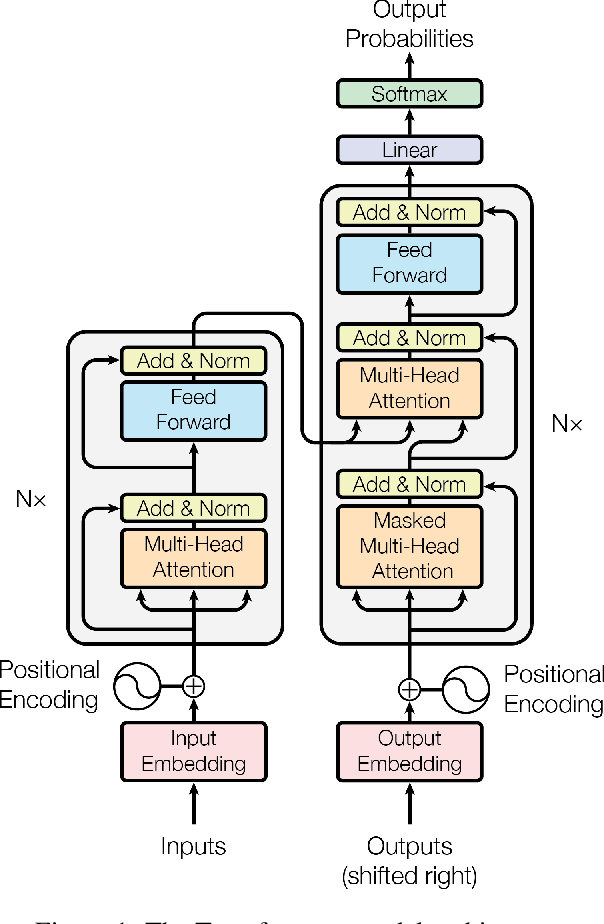
\includegraphics[width=0.5\linewidth]{Latex//sections//images/transformermodel.png}
        \caption{Transformer model architecture Vaswani et. all 2017}
        \label{fig:enter-label}
    \end{figure}

%TODO
\todo{add more, esp. more explainations}
\subsection{Cascaded Models}
Cascaded Speech translation Models consist of 2 parts a part that is responsible for transcribing the audio, which is usually done with an ASR model, and a part that is responsible for translating the resulting transcription, which is done with neural machine translation or statistical machine translation. 
%TODO citation and expand
\tikzstyle{block} = [rectangle, draw, text width=3.5cm, text centered, minimum height=1.2cm, fill=blue!20]
\tikzstyle{arrow} = [thick,->,>=stealth]
\tikzstyle{inputoutput} = [ellipse, draw, text width = 3.5cm, minimum height=1cm, text centered, fill=green!20]

\begin{figure}
    \centering
    

\begin{tikzpicture}
    
    % Nodes
    \node (input) [inputoutput] {Speech Input \\(Source Language)};
    \node (asr) [block, below of=input, node distance=3cm] {Automatic Speech \\ Recognition (ASR)};
    \node (translation) [block, right of=asr, node distance=5cm] {Text Translation \\ (e.g., MT model)};
    \node (output) [inputoutput, below of=translation, node distance=3cm] {Speech Output \\ (Target Language)};

    % Arrows (angled)
    \draw [arrow] (input) -- (asr);
    \draw [arrow] (asr) -- (translation);
    \draw [arrow] (translation) -- (output);

    % Labels for processes
    \node[below of=asr] {Speech Recognition};
    \node[below of=translation] {Text Translation};
    

\end{tikzpicture}
\label{fig:cascaded model}
\caption{Basic overview of a cascaded speech translation model}
\end{figure}
\subsection{End-to-End Models}
End-to-End Speech translation models do not have the explicit split between the Automatic Speech Recognition model and the translation, this means that such a model gets audio as an input and outputs the text in the target language. 
End-to-End models are trained to perform a task from the raw input, which in this case is audio, to the output, in this case the corresponding translation, without any intermediate processing from outside the model or feature-engineering in sub-models. 
%TODO citations, different architectures and expand
\subsection{Whisper}
Whisper is a multilingual multitask Model that is focused on speech processing and was proposes in the Robust Speech Recogintion via Large-Scale Weak Supervsion paper \cite{radford2022robust}. 
It's architecture is based on a classical Transformer Encoder-Decoder Architecture where the Transformer Encoder Blocks consist of self attention blocks and Multilayer perceptron blocks. 
The Transformer Decoder blocks use the learned position embeddings and tied input-output token representations. 
The encoder and decoder ahve the same number of transformer blocks .
The audio pre-processing is done by making sure the audio chunks that are then given to the model are 30 seconds long have ben sampled to 16,000 Hz and have a 80-channel log-magnitude Mel spectrogram repesentation, this log-mel spectrogramm is then computed with 25-milliseconf windows and a stride of 10 milliseconds. 
This input is then scaled to be between -1 and 1 and is but through 2 convolutional layers that have a filter width of 3 and use the GELU function as activation function, the second of those 2 layers has a stride of 2. 
The resulting data is then embedded with a sinusodial position embedding, which means %TODO
and put in the Encoder blocks. 

\begin{figure}
        \centering
        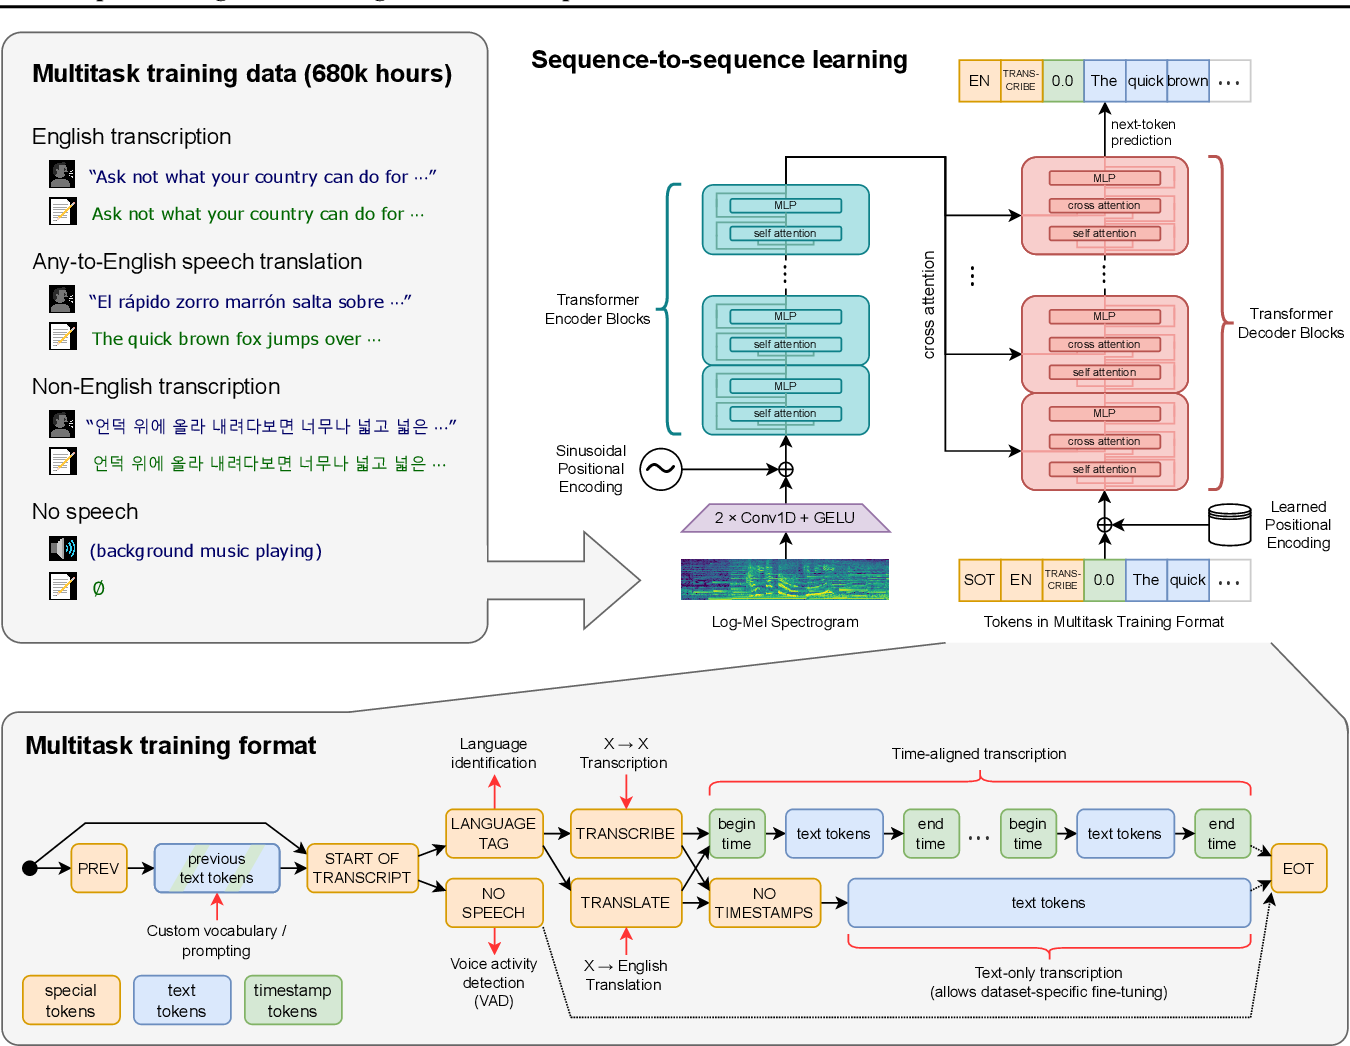
\includegraphics[width=0.5\linewidth]{Latex//sections//images/whispermodel.png}
        \caption{Overview of the Whisper architecture Radford et. al 2022}
        \label{fig:whispermodel}
    \end{figure}

%TODO
\subsection{Seamless}

Seamless is a Multimodal model 
experiments were run on \cite{seamless2023}, specifically the v2 large version which is an improved version of the SeamlessM4T model, 
of it both for the cascaded part and the end-to-end part

Seamless is a multilanagual multimodal model that uses a Transformer architecture. 
the architecture was proposed in \cite{seamless2023}
as the Transformer it is using a Encoder-Decoder architecture that in the v2 version uses a w2v-Bert speech encoder which was pretrained on unlabeled audio data. 
the general architecture is shown in \ref{fig:seamlessmodel}, for this thesis only the left half up to the Transformer Text decoder of the figure is relevant. 

\begin{figure}
        \centering
        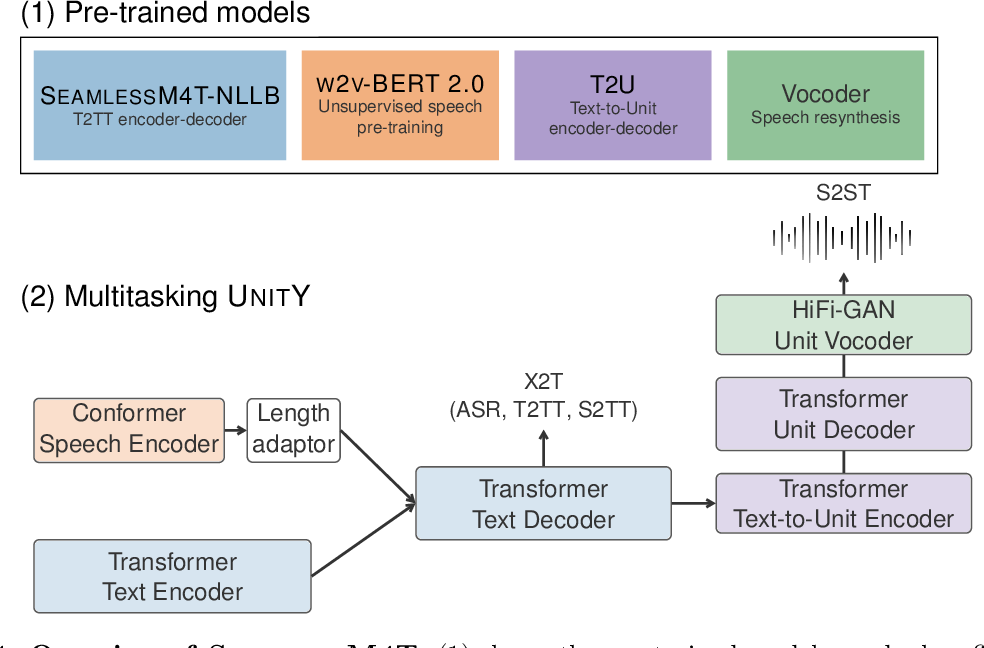
\includegraphics[width=0.5\linewidth]{Latex//sections/images/seamlessmodel.png}
        \caption{Overview of SeamlessM4T. (1) shows the pre-trained models used when finetuning multitasking UnitY. (2) outlines multitasking UnitY with its two encoders, text decoder, T2U encoder-decoder, and the supporting vocoders for synthesizing output speech in S2ST. \cite{seamless2023}(figure 4)}
        \label{fig:seamlessmodel}
\end{figure}
    
v2 uses a non autoregressive text to unit decoding which is the main difference to the first version however this change does not change much for this thesis as it only operates on Text-to-Text and Speech-to-text translation. 
The other change for v2 is that it uses a w2v-Bert 2.0 \cite{chung2021w2vbertcombiningcontrastivelearning} encoder that is trained self-supervised on 4.5 million hours of unlabled audio, as compared to the previous 1 million hours of unlabeled data. 
SeamlessM4T has been trained on unlabeled, human-labeled, pseudo-labled and automatically aligned data, where the text-to-text-translation (T2TT) was done on NLLB data \cite{nllbteam2022languageleftbehindscaling}
which is a method of creating low-resource language datasets with a combination of using flores \cite{guzmán2019floresevaluationdatasetslowresource} and NLLB Seed dataset, which is a set of professionally translated sentences in the wikipedia domain. 
% from seamless v2 paper
The X2T model, which can do T2TT, ASE and Speech to Text translation(S2TT), is trained on different sources of S2TT data that is human-labeled, pseudo-labeled and automatically aligned and is a combines the v2w-Bert model and the Text encoder from the NLLB T2TT model and the corresponding decoder.
It was trained in 2 steps on this data, the first one forcuses on supervised English ASR and S2TT data where the target langauge is English. 
The 2. step then focuses on english to X S2TT and non-English ASR data.


%TODO read further
\subsection{SentencePiece}
SentencePiece \cite{kudo-richardson-2018-sentencepiece} is a tokenizer and detokenizer that allows for subword units, especially byte pair-encoding \cite{sennrich-etal-2016-neural}, that are language independent as the sentences are treated as unicode character sequences and preprocessing is not always needed. 
It's comprised of a Normalizer, a Trainer, an Encoder and a Decoder. 
The Encoder uses the Normalizer to normalize the Test and then tokenizes the sentence. 
In the SentencePiece implementation the Decoding is considered the inverse operation of Encoding of normalized text, this results in a lossless tokenization, so there is no information loss over the process of encoding and decoding. 
To achieve this SentencePiece encodes white spaces with a meta-symbol that can be reverted. 
SentencePiece also manages the Vocabulary that is used in preprocessing as it also outputs a dictionary and can output a id sequence to text and vice versa mapping. 
As the SentencePiece model is self-contained it also leads to better reproducibility as only the model file is needed, which is publicly available. 

\subsection{DeltaLM}
DeltaLM is one of the current state of the art Neural Machine Translation models and the architectures that was proposed in \cite{ma2021deltalm}. 
It is based off of the classical Encoder-Decoder structure but both the encoder and decoder are initialised with the pretrained multilingual encoder. 
The training happens in a self-supervised manner. 

DeltaLM is considered one of the best text to text translation models. 

In addition to this is the Decoder a Interleaved Transformer Decoder, which is not the same architecture as the encoder and differs from the standard Transformer decoder in that the Transformerblocks now consist of a self-attention layer, two feed-forward networks and a cross-attention layer which are arranged as seen in \ref{fig:interleaved decoder}. 
This way of building the decoder is more similar to the structure of the encoder and makes it easier to leverage the pretrained encoder. 
The interleaved decoder is then initialised with the layers from the pretrained encoder, which is the InfoXLM \cite{chi2021infoxlminformationtheoreticframeworkcrosslingual}, in the following way, the self-attention and the bottom FFN layers are initialised wiht the odd layers of the InfoXLM encoder and the cross-attention and top FFN layers are initialised with the even layers. 
The leftover components of the decoder are also initialised the same as the pretrained encoder. 
This means that all of the sublayers are initialised with the pretrained weights and none of them use randomised names. 

%TODO
\begin{figure}
    \centering
    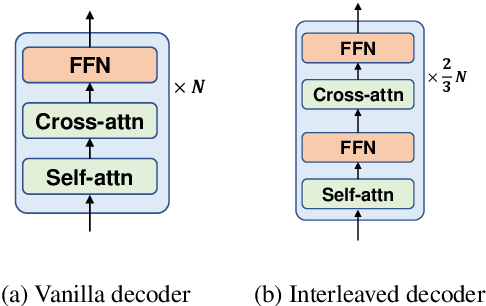
\includegraphics[width=0.5\linewidth]{Latex/sections/images/interleaveddecoder.png}
    \caption{Vanilla Transformer Decoder (left) compared to the interleaved Transformer decoder(right) from Ma et. al 2021}
    \label{fig:interleaved decoder}
    %source dlm paper
\end{figure}

\chapter{Related works}
\label{ch:relatecworks}
Simmilar works have been done for ASR with \cite{8683086}
\cite{negri-etal-2014-quality}

and on a full scale by 
\cite{le2016automatic} which is a supervised approach that classifies on a word basis rather than a segement basis


\chapter{Methodology}\todo{move around to have section with fomicheva proposed methods, and my own proposed methods, like how to apply the fomicheva methods to ASR, how to combine them etc.}
\label{ch:methods}
This chapter goes more in depth on how the Quality estimation scores are derived from data retrieved from the models in general, whereas chapter \autoref{ch:experiment} goes more in depth on how it was done for the specific models and some of the potential errors that were made in the experiments.
%\todo{how to derive the QE scores from the approaches like log probability or dropout,... }
%\todo{all in a more mathematical sense -> maybe move stuff from background here}

\section{Translation and transcription}
The general formula of both the translation and transcription probability is $$TP=-\frac{1}{T}\sum_{t=1}^T log\; p(y_t) \label{formula:translation Probability}$$
where p is the log-probability of generating the t-th token in the output sequence, so to get the probability of the whole sequence log-probabilities the log-probabilities of each token are added together, and then normalized with the length of the sequence T. 
This is the case since the architectures are the same.
These log-probabilities are the probabilities after applying the softmax to the decoding probability distribution and then applying the logarithm to the highest probability.
The sum of those values is then used as the quality estimation, especially as a baseline to compare the other estimators to.
%- this is the baseline and the easiest measure to acquire
%- take the softmax values at the last layer of the model to estimate quality (normal mode) for transcription and translation 


\subsection{Transcription probability}
The transcription probability is the probability that the ASR component transcribes the audio to this sequence of text $y_1\dots y_n$. 
In encoder-decoder models this is most commonly done by encoding the audio signal in the encoder and then, using attention mechanisms to get the context for the current next output token and then using previous predicted tokens to decode the current token. 
That next output token has a certain probability that, after applying the softmax to the whole probability distribution of the Vocabulary is between 0 and 1. This probability is on the last layer of the decoder and retrieved from the model. 
This probability can be mathematically described in the formula $$p(y|x,\Theta)=\prod_{t=1}^T p(y_t|y_{<t}, x, \Theta) $$ where $\Theta$ is the model parameters, x is the audio input sequence, the softmax is used after every decoding step t on the resulting probability distribution $p(y_t|y_{<t}, x,\Theta)$. 
\todo {add reference?, check with bayes in background}

\subsection{Translation probability}
The translation probability is the probability a Machine translation model out puts the sequence $y = y_1, y_2 \dots y_n$ for the input $x=x_1, x_2 \dots x_n$. The probability is calculated by Formula \autoref{formula:translation Probability} where the probability of generating the sequence y is defined as $$ p(y)=p(y|x,\Theta)=\prod_{t=1}^T p(y_t|y_{<t}, x, \Theta)$$ where $\Theta$ is the model parameters.
The probability $p(y_t|y_{<t}, x,\Theta)$ is the probability distribution after the decoding step of the t-th decoding step after applying the softmax.
The $\frac{1}{T}$ is there to normalise the translation probability over the length of the translation sequence T as to minimize the effect of longer sequences getting a higher score when they shouldn't. 
\todo{add reference? check with bayes}


\subsection{Softmax Entropy}\label{sect:entropy}
The Softmax entropy is the entropy of each element in the vocabulary at decoding step, this is a way to measure the uncertainty in the vocabulary at each decoding step.
To compute the entropy \autoref{entropy} for each element, and then sum all entropies in the Vocabulary together, this results in the entropy of the decoding step. 
Then the sum of the entropy of all decoding steps is taken and normalised over the sequence length. 

This results in the Formula:
$$\text{Softmax-Entropy}=-\frac{1}{T}\sum_{t=1}^T\sum_{v=1}^V p(y_t^v)log\; p(y_t^v) \label{formula:translation entropy}$$ where V is the Vocabulary size and T is he length of the generated sequence. The minus comes from the entropy and is only moved in front of the sums for ease of computation.
Due to how entropy works a lower value, so one closer to 0, in the score is better since then the information that the vocabulary contains less entropy when there is less uncertainty. so if there are less entries in the vocabulary that have similar probabilities during a single decoding step then the entropy of that decoding step will be lower.

\subsection{Standard Deviation}\label{sect:stddiv}
The standard deviation, similarly to the Softmax entropy aims to measure the uncertainty by looking at the dispersion of the probabilities in the sequence. 
Since the mean that is the probability score does not account for the different behaviour that for example [0.1,0.9] and [0.5,0.5] have even though the have the same mean. 
To obtain this quality estimator the standard deviation over the top token at each decoding step of a sequence is computed.
This means the mathematical formula is: $$\text{Seq-Std}=\sqrt{\mathbf{E}[P^2]-(\mathbf{E}[P])^2}$$ where $P=p(y_1) , \dots p(y_T)$ is the token-level log-probabilities for the sequence.
\todo{expand? explain how the std div works?}

\section{Dropout}
Dropout, in particular the Monte Carlo dropout \cite{gal2016dropoutbayesianapproximationrepresenting}, which is the masking of neurons to 0 based on a Bernoulli distribution, aims to measure the uncertainty in a Deep Neural network. 
For this the same input is run N times through the model, due to the potential masking of neurons different results can be observed from the model. Based on how much these results differ from each other and a reference that was obtained without dropout conclusions can be made as to how certain the original result is. 
The following measures have been used in the past to minimize the effect of low quality outputs on neural machine translation training with back translation \cite{wang-etal-2018-alibaba}
The dropout measures are used on the transcription and translation part of the cascaded models. 


\subsection{General Probability}
\label{dropoutprob}
The dropout probability is the mean of the regular probabilities, as done in \autoref{transcription results}. 
For this the method described above is run on the model with dropout several times and get the Probability scores for each run. 
This results in the formula:
$$\text{D-TP}=\frac{1}{N}\sum_{n=1}^N TP_{\hat\theta n}\label{formula:dropoutprobability}$$
This method works to estimate the quality because if the masked neurons affect the result sequence and resulting probability, especially if the model is very uncertain about the resulting sequence. if the model is certain about the resulting sequence then masking neurons to 0 will not affect the resulting sequence and probability as much. 

\subsection{Variance}
\label{dropoutvar}
The dropout variance is the variance of the different probabilities gathered during the N runs. 
Mathematically this can be described as:
% measures the uncertainty of the N runs 
$$\text{D-Var}=E[TP_{\hat\theta}^2]-(E[TP_{\hat\theta}])^2\label{formula:dropoutvariance}$$
Where $TP_{\hat\theta}$ is the probability \autoref{formula:translation Probability} of the runs. 
If the Dropout Variance is high then the model is uncertain about the resulting sequence, and if the variance is closer to 0 it is quite certain about the sequence.
So a low variance is to be considered better than a high score.

\subsection{Combo}
As the variance does not take into account the probability of the sequence, a combination of the dropout Probability and dropout variance is proposed by Fomicheva et al \cite{fomicheva2020unsupervised}. 
The combination of the results from the probability and the variance is done by calculating $$D-Combo=(1-\frac{D-TP}{D-Var})\label{formula:Dropoutcombo}$$, where $D-TP$ and $D-Var$ are the Translation probability mean (\autoref{dropoutprob}) and the Dropout variance (\autoref{dropoutvar}).



%\subsection{Lexical Simililarity}
\section{unified score}
The unified score is a combination score for the transcription and translation part as an attempt to approximate the quality of the whole cascaded model. 
For this the translation probability and transcription probability are multiplied together as both the translation and transcription probabilities fall between 0 and 1. 

$$\text{unified score}= TP_{transcript}\cdot TP_{translation}$$

alternative options for a unified score are weighing the translation and transcription probabilities differently, which results in the formula $$unifiedscore_\alpha= (1-\alpha) TP_{transcript} \cdot (\alpha)TP_{translation}$$. 
This was previously proposed in by Le et al. \cite{le2016automatic}, but in that case the quality estimation is done with classification onto good or bad translations and not scores.


%\chapter{the Dataset}
\label{ch:Dataset}
The used dataset for all the scores is the benchmark section of the IWSLT2023 \cite{sperber2024evaluating}, which consists of TED talks and contains both reference translations and reference transcriptions, as well as a segmentation for the transcriptions, which matches roughly the translation segmentation. 
\section{Segmentation}
\label{sec:FirstContent:Segmentation}
Since most ASR models and end-to-end speech translation models only take audio up to a certain length as input the given audio files have to be segemented into smaller chunks. 
The segmentation of the audio from the data set will be done with the timestamps given in the dataset itself. The timestamps given in the dataset correspond to the source language transcription reference and the target language translation also correspond mostly well with the reference segments given in the dataset. 
For the segments that do not overlap properly or are shifted by a segment in the given xml, mwerSegementer is used to align the outputs with the references properly, so the comet scores can be calculated on those alrigned sentences and the computed reference scores fit. 
mwerSegmenter minimises the WER between 2 segments,  for this the model transcription or translation is used as the gold segmentation to which the reference is aligned 
%% Karlsruhe Institute of Technology
%% Institute for Anthropomatics and Robotics (IAR)
%% Artificial Intelligence for Language Technologies (AI4LT) lab
%%
%% Prof. Dr. Jan Niehues
%% Lab's website https://ai4lt.anthropomatik.kit.edu/english/index.php

\chapter{Experiments}
\label{ch:experiment}
This chapter details the dataset and the experiments that have been run on Whisper \cite{radford2022robust}, Seamless \cite{seamless2023} and DeltaLM \cite{ma2021deltalm}.
The experiments on whisper and seamless have been made with the help of the huggingface \cite{huggingfaceseamless}\cite{huggingfacewhisper}\footnote{huggingface can be found here: \url{https://huggingface.co/}, the whisper model documentation here: \url{https://huggingface.co/docs/transformers/model_doc/whisper} and the Seamless M4T v2 documentation here: \url{https://huggingface.co/docs/transformers/main/model_doc/seamless_m4t_v2}} models and frameworks, whereas DeltaLM\footnote{the code for deltaLM can be found here: \url{https://github.com/microsoft/unilm/tree/master/deltalm}} has been used with the fairseq toolkit \cite{ott2019fairseqfastextensibletoolkit}\footnote{the documentation for fairseq can be found here: \url{https://fairseq.readthedocs.io/en/v0.10.2} and the github repo is found here: \url{https://github.com/facebookresearch/fairseq}}.

For the cascaded models the transcription from the ASR model is passed into the translation model. 
In the case of the dropout quality estimators the decision of which transcript to put into translation model has been made based on the quality estimations of those transcriptions.
One option is taking the transcript with the highest transcription probability mean to be the basis for the dropout of the translation. 
This is not the best way of obtaining the best transcription as the basis for the translations but it is a very good method if only the dropout part of the quality estimation is run. 
An example of this can be seen in \autoref{tab:transcriptshift}.
This is the case as there are some transcriptions with dropout that have a higher score at the end than the regular transcript would have, but have obvious signs of the dropout being enabled, like a lot of repeated letters.
So taking the transcript with the highest score can propagate unwanted errors in the transcription to the translation section.
The other and better method of obtaining a good transcript is running the transcription once without the dropout turned on, as that would result in the regular transcript that the model would output, but this method is fairly likely to return such a transcription due to the way of how the dropout is used. More on that is described in \autoref{experiment:dropout}.
Running the transcription once more without using dropout should be considered as compared to the number of runs that is done for the dropout it does not add a lot more time to the runtime of a single sequence.
\begin{table}[ht]
    \centering
    \begin{tabularx}{\textwidth}{l|X}
         qe& transcript \\\hline
         -0.30165& Because that's it. \\
         -0.12921& Because that's it.\\\hline
         -0.33879& No, no, no, no, no, no, no, no, no, no, no, no, no, no, no, no, no, no, no, no, no, no, no, no, no, no, no, no, no, no, no, no, no, no, no, no, no, no, no, no, no, no, no, no, no, no, no, no, no, no, no, no, no, no, no, no, no, no, no, no, no, no, no, no, no, no, no, no, no, no, no, no, no, no, no, no, no, no, no, no, no, no, no, no, no, no, no, no, no, no, no, no, no, no, no, no, no, no, no, no, no, no, no, no, no, no, no, no, no, no, no, no, no, no, no, no, no, no, no, no, no,, no, no, no, no, no, no, no, no, no, no, no, no, no, no, no, no, no, no, no, no, no, no, no, no, no, no,, no,, no, no, no,, no, no, no, no, no, no, no, no, no, no, no, no, no, no, no, no, no, no,. no, no, no, no, no, no, no, no, no, no\\
         -0.094421 &Not a model, not a replica.\\
         -0.644232&  Not a model, not a replica.
    \end{tabularx}
    \caption{Example of differing transcript results, the top is an example where the transcript with dropout (first line) that has the highest quality estimation score is the same as the transcript without dropout. Compared to an example where the transcription withe highest score is vastly different from the non dropout transcription, 2. to last line. The last line is a different result from the dropout runs that is essentially the non dropout result. The left column is the corresponding quality score; the quality score shown is the transcription mean.}
    \label{tab:transcriptshift}
\end{table}

\chapter{the Dataset}
\label{ch:Dataset}
The used dataset for all the scores is the benchmark section of the IWSLT2023 \cite{sperber2024evaluating}, which consists of TED talks and contains both reference translations and reference transcriptions, as well as a segmentation for the transcriptions, which matches roughly the translation segmentation. 
\section{Segmentation}
\label{sec:FirstContent:Segmentation}
Since most ASR models and end-to-end speech translation models only take audio up to a certain length as input the given audio files have to be segemented into smaller chunks. 
The segmentation of the audio from the data set will be done with the timestamps given in the dataset itself. The timestamps given in the dataset correspond to the source language transcription reference and the target language translation also correspond mostly well with the reference segments given in the dataset. 
For the segments that do not overlap properly or are shifted by a segment in the given xml, mwerSegementer is used to align the outputs with the references properly, so the comet scores can be calculated on those alrigned sentences and the computed reference scores fit. 
mwerSegmenter minimises the WER between 2 segments,  for this the model transcription or translation is used as the gold segmentation to which the reference is aligned 

\section{Models}
More details on the models used in the experiments. More information on the implementations, like how the scores are retrieved in specific, can be found in \autoref{ch:implementation information}. For Whisper and seamless the scores are retrieved with the help of functionality from huggingface or pytorch; for DeltaLM it's functionality from fairseq where available. More on that is found in the models section.

\subsection{Whisper}
The Transcription step is only done on the Whisper model.
Open AI gives several different sizes for Whisper models. In this thesis the medium model is used, specifically the pretrained model that is available on huggingface, which provides a processor and a few different Whisper models that have a different head on top of it.
The basic Whisper model on huggingface outputs the raw hidden states without a specific head on top of it. 
The specific model version used in the experiments is the WhisperForConditionalGeneration, as it has a language modelling head, and is recommended for automatic speech recognition. There are also ones that have heads for audio classification or a language modelling head that is a linear layer with weights tied to the input embeddings. 
 
\subsection{DeltaLM}
The experiments \cite{ma2021deltalm} were done on a fine tuned large version of DeltaLM that was fine tuned using the training data from the IWSLT 2023 constrained category. For this only the English-German part was used.

The text was preprocessed with the pretrained SenctencePiece model and dictionary that has been provided on the DeltaLM github page \cite{deltalmurl}. After that it is preprocessed with faireq preprocess. The result of this is then put into fairseq generate with batch size and beam size 1. 

 Running the experiments was done with the help of the fairseq toolkit \cite{ott2019fairseqfastextensibletoolkit} which returns the probability of the specific translation along with the translation hypothesis, and prints the softmax probabilities of the top token after each decoding step. By default these probabilities are in the base 2 logarithm. 

 
\subsection{Seamless}
There are a couple of difference model sizes of seamless that are provided by Meta. The one that was used to run the experiments is the seamless M4T v2 large model that is available on huggingface. Similarly to the Whisper model, the seamless models on huggingface also have several more specialized models. 
For the text translation the seamless v2 large model used is the SeamlessM4Tv2TextToText model.
For the end-to-end translation the SeamlessM4Tv2SpeechToText model is used. 

\section{Dropoutless Experiments}
The first of the experiments is to retrieve the non dropout scores from the different models. For the cascaded models this means retrieving or calculating both of the transcription scores, the translation score, the softmax entropy, and the standard deviation for the token probabilities. 
For the spoken language translation end-to-end model this means calculating the translation probability, the softmax entropy, and the standard deviation of the token probabilities.

%In the end-to-end translation there is no intermediate step between the audio and text part so the resulting probability is a single score for the whole process.
%The resulting probability formula comes from the architecture, which in this case is a encoder decoder architecture which results in the formula: $$-\frac{1}{T}\sum_{t=1}^T log\; p(y_t)$$ which is the same as the translation probability and the transcription probability.

To get the softmax entropy from the models the batch and beam size are set to 1 as otherwise the resulting tensors make it more difficult to pick out which is the right entropy for the resulting batch. 


\section{Dropout}\label{experiment:dropout}
To run the the dropout based experiments 30 forward passes with the same input are used on the models. 
Each time, neurons in the model are masked to 0 by some probability, which is usually the same probability as was used in training, or set to 0.1 when no information about that was available. The 0.1 dropout probability is used on both Whisper and seamless during training, so using the same probability on DeltaLM only makes sense. 

Due to the nature of pytorch and huggingface models, the dropout has to be done in training mode, as the evaluation mode turns off any dropout layers that are in the model. Due to this and a bug in the implementation for caching during forward passes in the seamless models on huggingface, which leads to a tuple index out of range error that only appears in training mode with dropout turned on, the caching was turned off in the seamless configurations for the dropout based experiments. This means caching is turned off on both the text translation and speech translation system.

\section{Unified Scores}
Different unified scores are calculated with the scores that have been retrieved in the previous 2 experiments for the cascaded models. To calculate the scores the unified score methods proposed in \autoref{methods:unified scores} are used. 
For this both the transcript probability score and the transcript mean score are paired with each of the regular translation scores. 
The gathered dropout scores are also combined, where the dropout transcription probability score and the dropout transcription mean are combined with the dropout translation probability, the dropout transcription variance scores are combined with the dropout translation variance score, and the dropout transcription combination scores are combined with the dropout translation combination score.

%% Karlsruhe Institute of Technology
%% Institute for Anthropomatics and Robotics (IAR)
%% Artificial Intelligence for Language Technologies (AI4LT) lab
%%
%% Prof. Dr. Jan Niehues
%% Lab's website https://ai4lt.anthropomatik.kit.edu/english/index.php

\chapter{Evaluation}
\label{ch:Evaluation}

%% -------------------
%% | Example content |
%% -------------------
\dots

\section{First Section}
\label{sec:Evaluation:FirstSection}

\dots

\section{Second Section}
\label{sec:Evaluation:SecondSection}

\dots

\section{Third Section}
\label{sec:Evaluation:ThirdSection}

\dots
%% ---------------------
%% | / Example content |
%% ---------------------
%% Karlsruhe Institute of Technology
%% Institute for Anthropomatics and Robotics (IAR)
%% Artificial Intelligence for Language Technologies (AI4LT) lab
%%
%% Prof. Dr. Jan Niehues
%% Lab's website https://ai4lt.anthropomatik.kit.edu/english/index.php

\chapter{Conclusion}
\label{ch:Conclusion}

\dots

%% --------------------
%% |   Bibliography   |
%% --------------------

%% Add an entry to the table of contents for the bibliography
\printbibliography[heading=bibintoc]

%% ----------------
%% |   Appendix   |
%% ----------------
\appendix
%% Karlsruhe Institute of Technology
%% Institute for Anthropomatics and Robotics (IAR)
%% Artificial Intelligence for Language Technologies (AI4LT) lab
%%
%% Prof. Dr. Jan Niehues
%% Lab's website https://ai4lt.anthropomatik.kit.edu/english/index.php

\iflanguage{english}
{\chapter{Appendix}}    % english style
{\chapter{Anhang}}      % german style
\label{chap:appendix}


%% -------------------
%% | Example content |
%% -------------------
\section{First Appendix Section}
\label{sec:appendix:FirstSection}
		
\setcounter{figure}{0}
		
\begin{figure} [ht]
  \centering
  \caption{A figure}
  \label{fig:anotherfigure}
\end{figure}


\dots
%% ---------------------
%% | / Example content |
%% ---------------------

\end{document}
